\documentclass{beamer}
\usepackage[ngerman]{babel}
\usepackage[utf8]{inputenc}
\usetheme{Boadilla}

\usepackage{multicol}
\usepackage{siunitx}

\begin{document}
\title{Information und Daten}
\subtitle{Grundlagenfach Informatik}
%\subtitle{Freifach Informatik}
%\subtitle{Berufsfeldfach Informatik}
%\subtitle{Ergänzungsfach Informatik}
\author{Oliver Probst (pro@kwse.ch)}
\institute{KSWE}
\date{11. August 2022}
\titlegraphic{
\includegraphics[scale=0.5]{graphics/kswe_logo.pdf}}

\begin{frame}
\titlepage
\end{frame}

\frame[c]{\frametitle{Information}\framesubtitle{Was ist Information?}

\begin{definition}[Information]
	Eine Information sind Daten mit einer Bedeutung. Dies kann ein gesprochener oder geschriebener Text sein, ein Bild, ein Geräusch, ein Duft oder eine Empfindung sein. Wir können diese Informationen mit unseren Sinnesorganen wahrnehmen und durch technische Hilfsmittel speichern oder übertragen.
\end{definition}

Beispiele:
\begin{itemize}
\item The quick brown fox jumps over the lazy dog.
\item Fahrplan der Bushaltestelle
\item Ein Bild
\end{itemize}
}

\frame{\frametitle{Daten}\framesubtitle{Was sind Daten?}
\begin{definition}[Daten]
Messwerte, Fakten, Gegebenheiten oder Zeitpunkte bezeichnen wir als Daten. Sie bestehen aus Ziffern, Buchstaben und Sonderzeichen oder werden durch eine Funktion beschrieben und sind meist mit einer Einheit versehen.
\end{definition}
Beispiele:
\begin{multicols}{2}
\begin{itemize}
\item \qty[per-mode = fraction]{90}{\km\per\hour}
\item \qty{1,99}{\kg}
\item \qty{128}{\giga\byte}
\item Alice
\item 4. Mai 1977
\item 1875 positive PCR-Tests
\end{itemize}
\end{multicols}
}

\frame{\frametitle{Daten}\framesubtitle{Was sind analoge Daten?}
\begin{definition}[Analoge Daten]
Beschreibt eine kontinuierliche Funktion (auch stetige oder stufenlose Funktion genannt) einen Vorgang, dann handelt es sich um analoge Daten. Somit existiert zu jedem Zeitpunkt ein Wert mit einer beliebigen Genauigkeit. Bei einem analogen Vorgang können prinzipiell unendlich viele verschiedene Werte vorkommen.
\end{definition}
}

\frame{\frametitle{Analoge Daten}\framesubtitle{Beispiel 1}
\begin{figure}[htb]
\centering
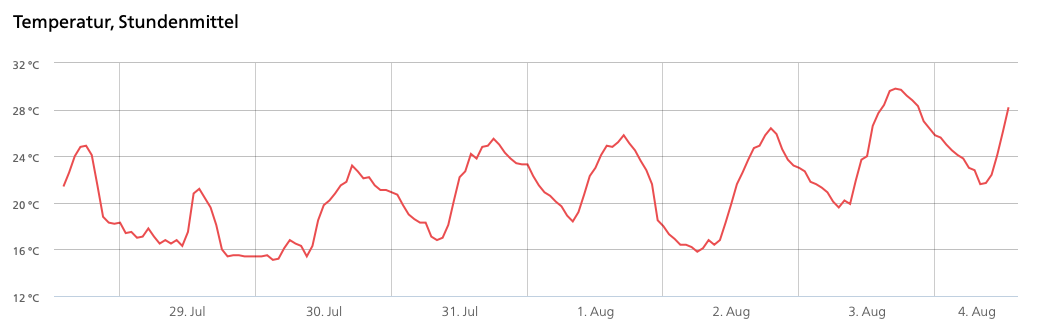
\includegraphics[width=\linewidth]{graphics/temperaturverlauf.png}
\caption{Temperaturverlauf an der Messstation Lägern ($845$ Meter über Meer) von MeteoSchweiz.}
\label{figure-temperaturverlauf}
\end{figure}
}

\frame{\frametitle{Analoge Daten}\framesubtitle{Beispiel 2}
\begin{figure}[htb]
\centering
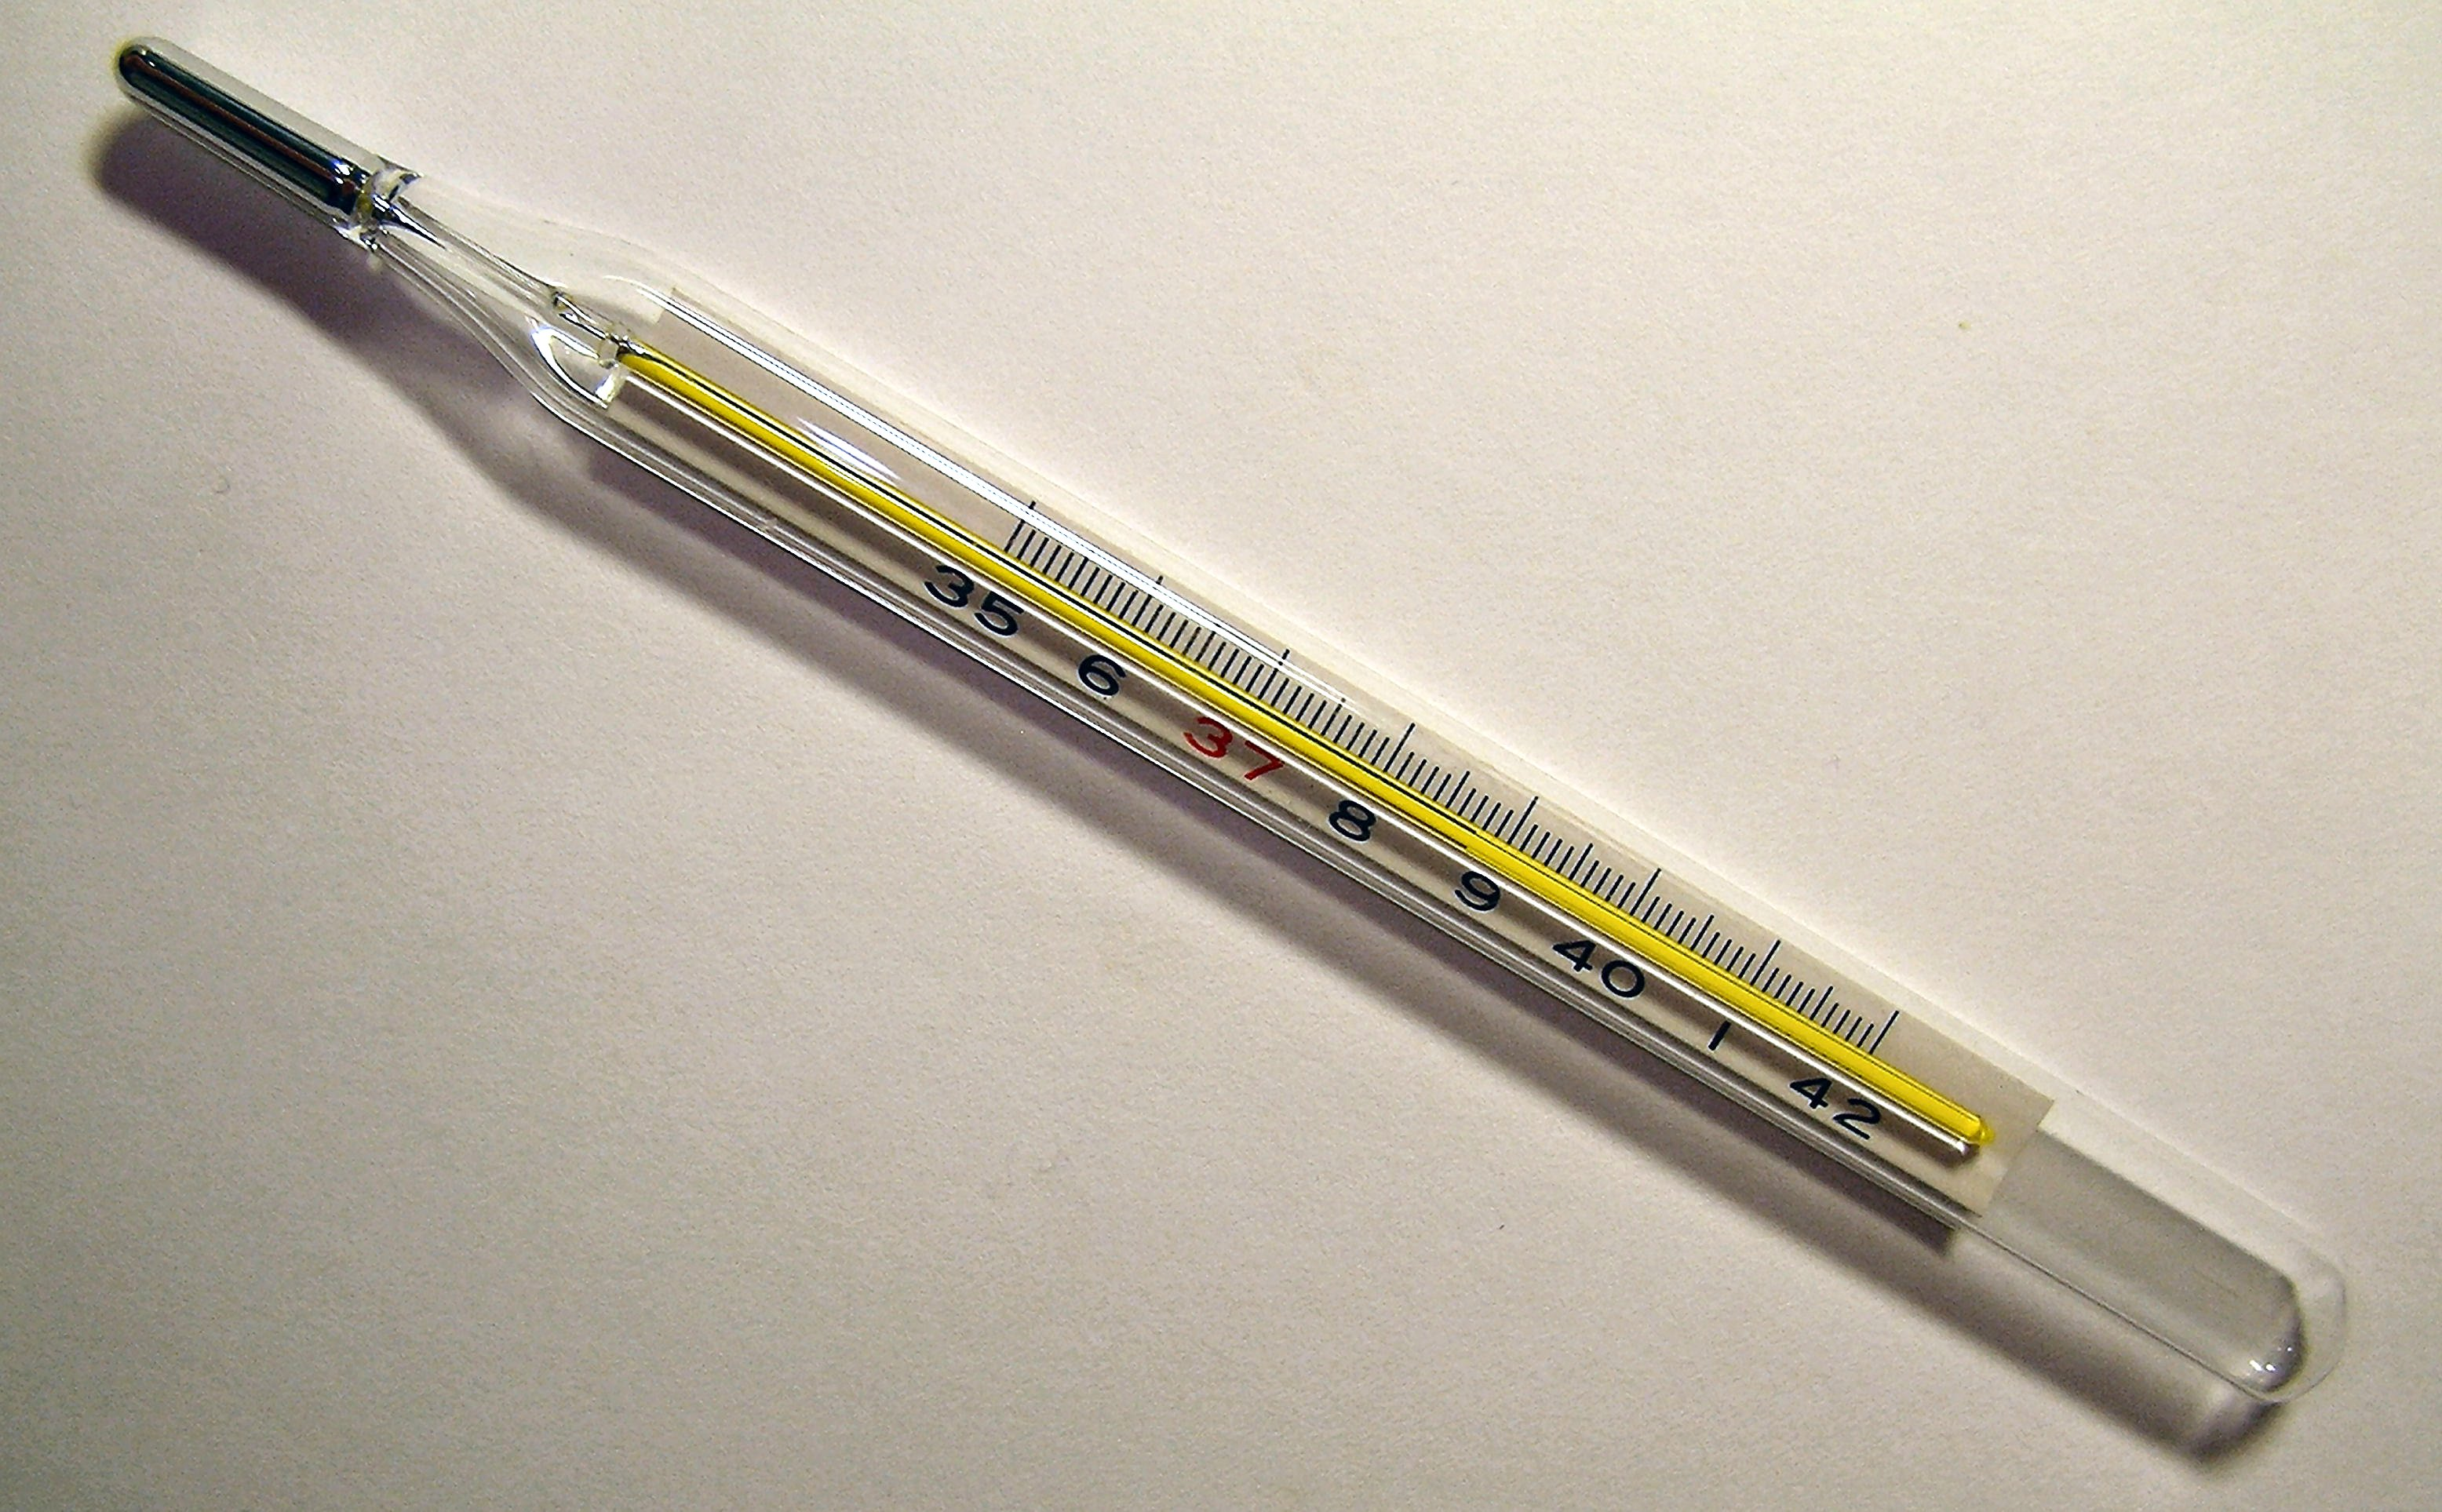
\includegraphics[width=0.75\textwidth]{graphics/qucksilberthermometer.jpg}
\caption{Klassisches Quecksilberthermometer zur Messung der Temperatur.}
\label{figure-quecksilberthermometer}
\end{figure}
}

\frame{\frametitle{Analoge Daten}\framesubtitle{Beispiel 3}
\begin{figure}[htb]
\centering
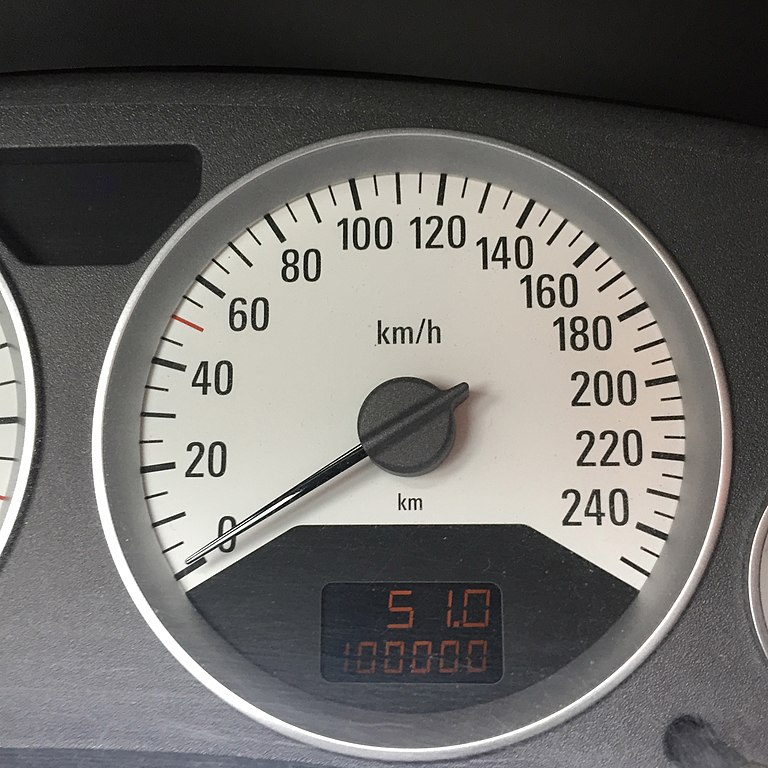
\includegraphics[width=0.5\textwidth]{graphics/tacho.jpg}
\caption{Tachometer mit analoger Geschwindigkeitsanzeige.}
\label{figure-tacho}
\end{figure}
}

\frame{\frametitle{Daten}\framesubtitle{Was sind digitale Daten?}
\begin{definition}[Digitale Daten]
Werden Daten nur durch eine Folge von Zeichen dargestellt, dann handelt es sich um digitale Daten.
\end{definition}
}

\frame{\frametitle{Digitale Daten}\framesubtitle{Unerwartetes Beispiel 1}
\begin{figure}[htb]
\centering
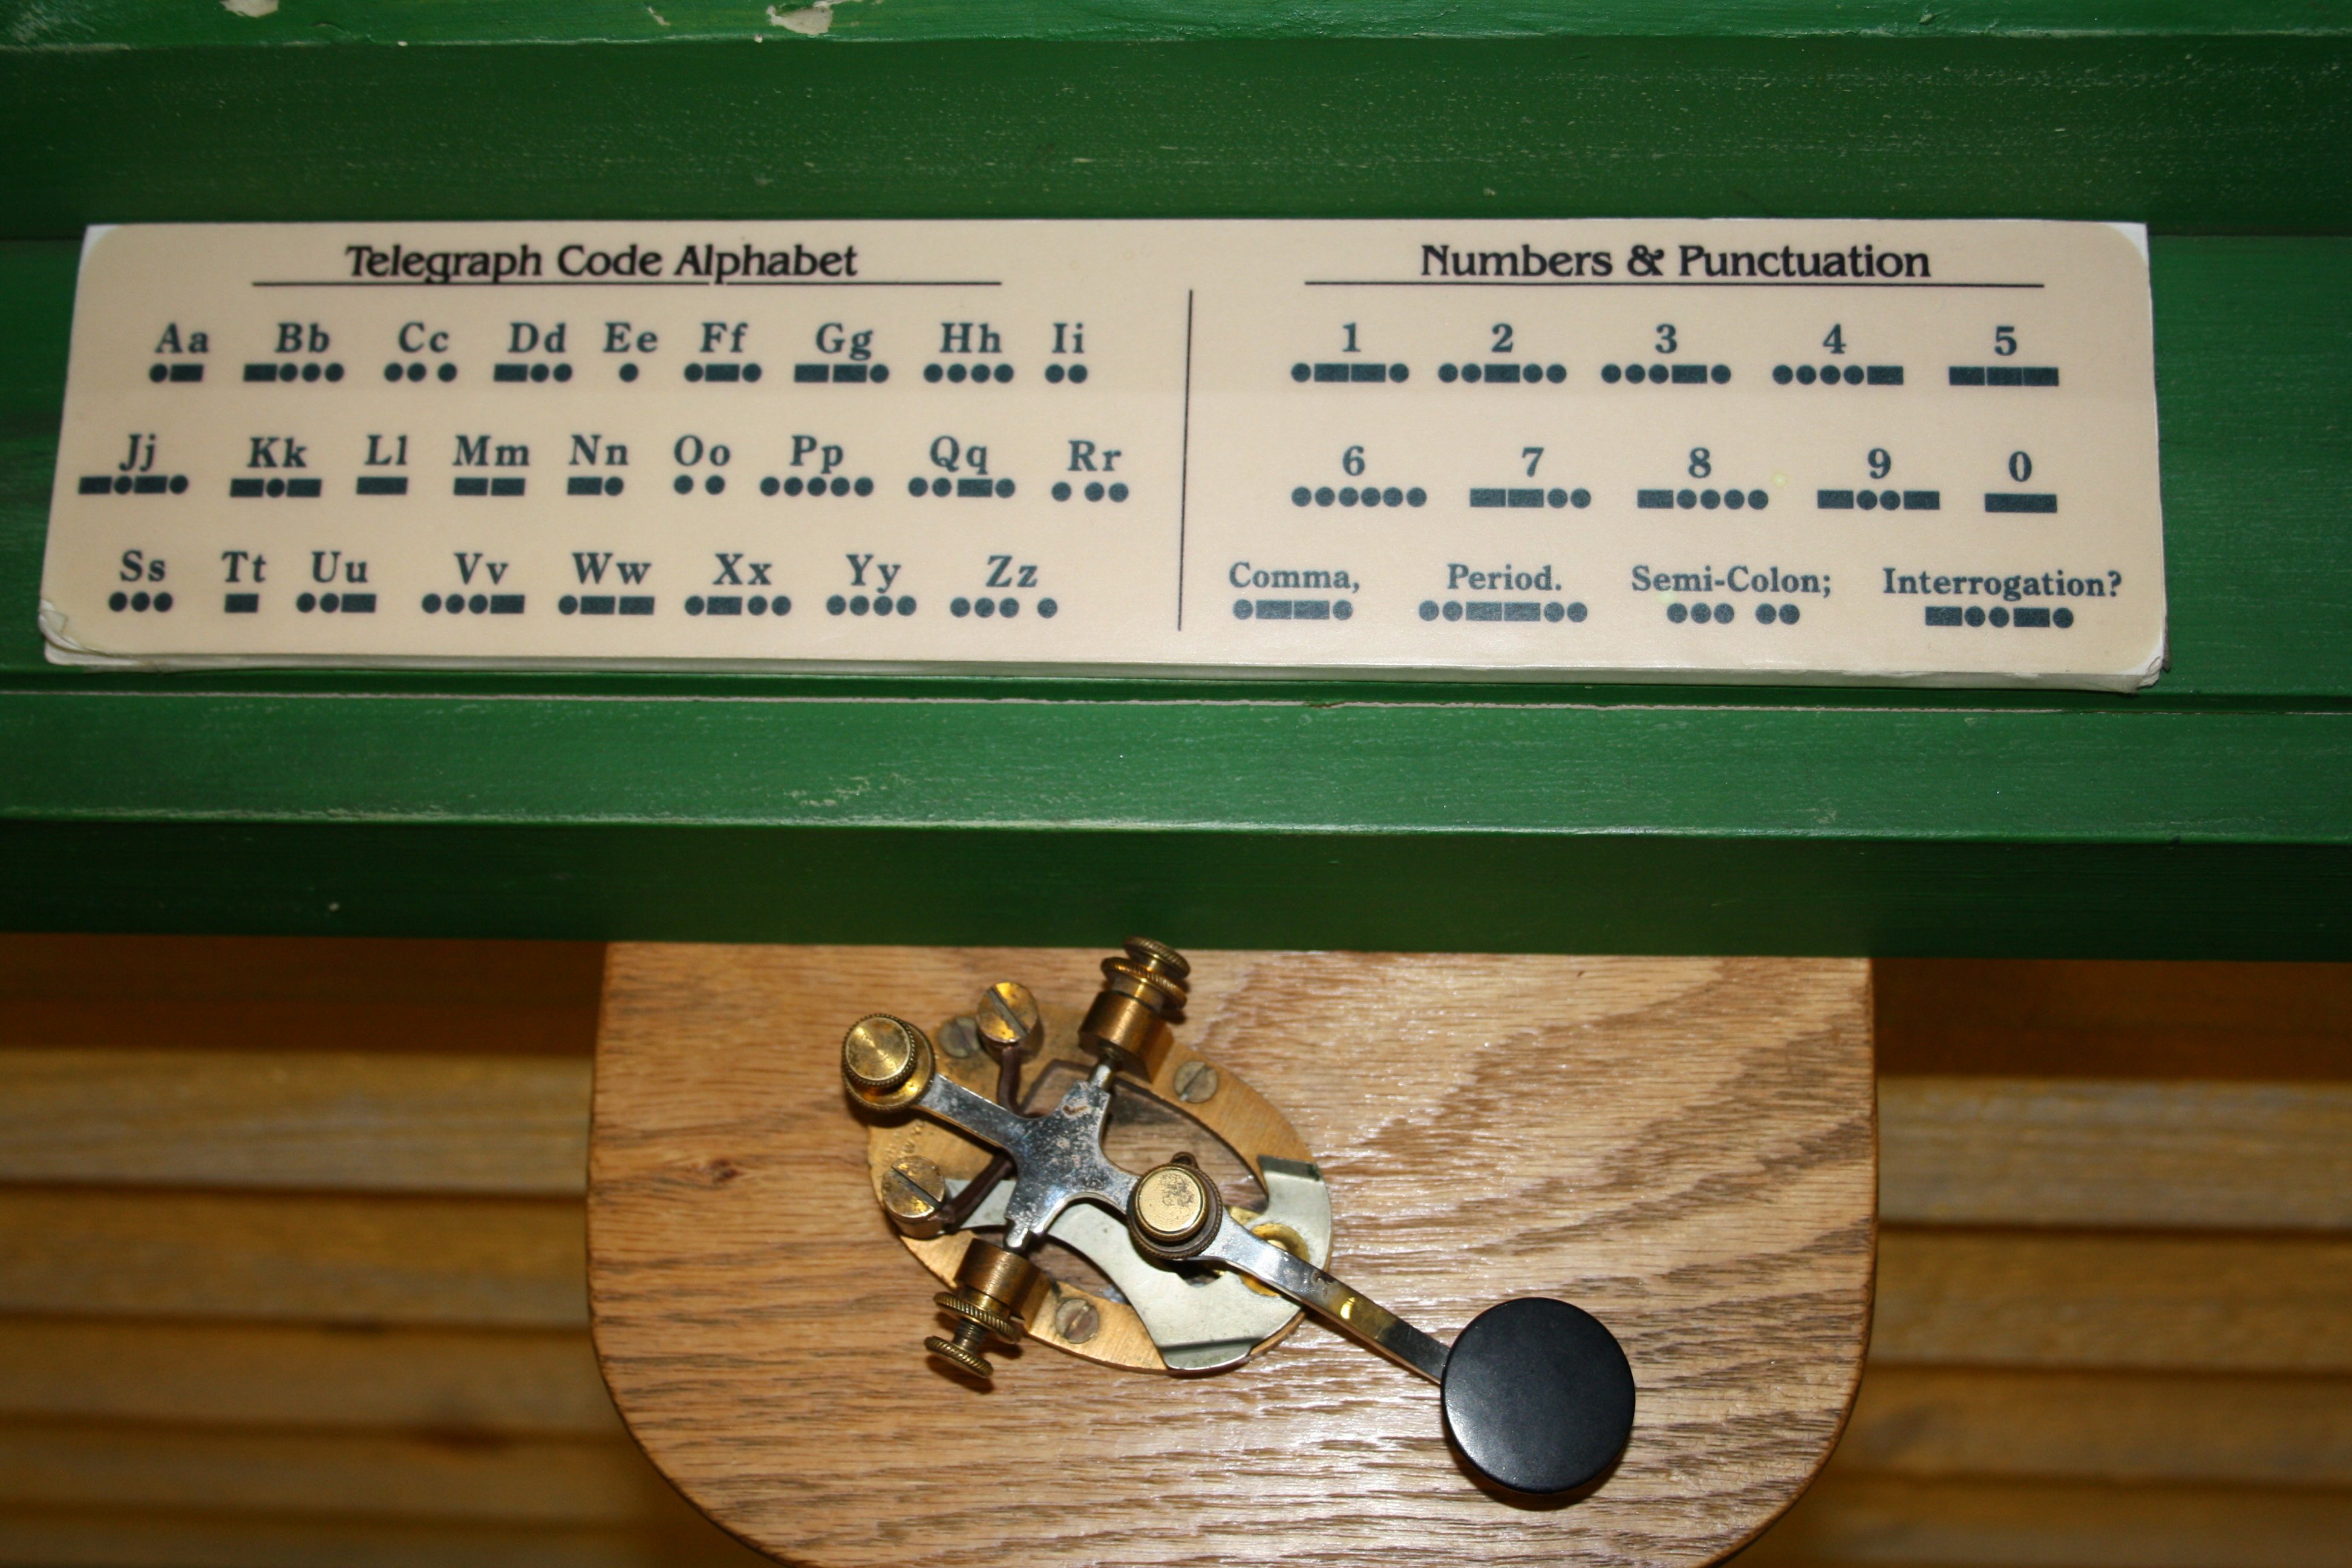
\includegraphics[width=0.6\textwidth]{graphics/morsecode.jpg}
\caption{Morsecode}
\label{figure-tacho}
\end{figure}

Beispiel: \url{https://de.wikipedia.org/wiki/Datei:SOS_morse_code.ogg}
}

\frame{\frametitle{Digitale Daten}\framesubtitle{Unerwartetes Beispiel 2}
\begin{figure}[htb]
\centering
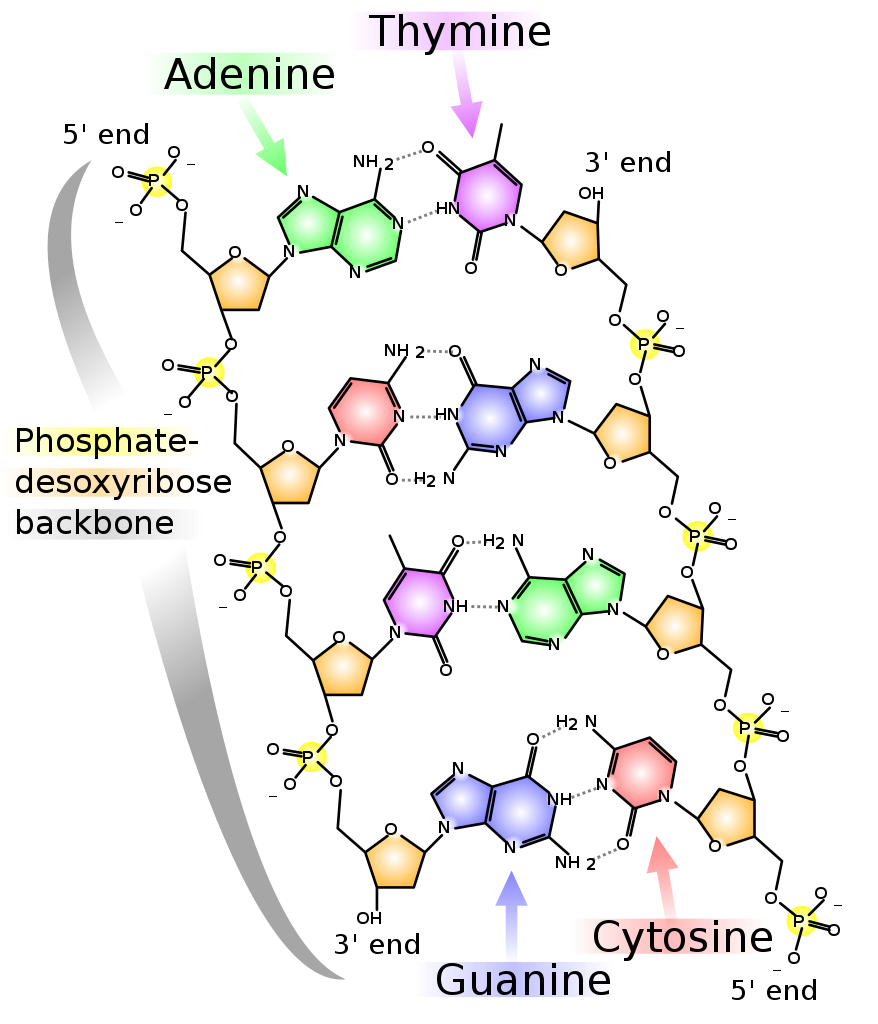
\includegraphics[width=0.35\textwidth]{graphics/dna.png}
\caption{DNA}
\label{figure-dna}
\end{figure}

Beispiel für eine DNA-Sequenz: ATG CGC AAT GCG ATA TAC
}

\frame[t]{\frametitle{Digitale Daten}\framesubtitle{Was sind Binärdaten?}
\begin{definition}[Binärdaten]
Digitale Daten die nur aus den Ziffern $0$ und $1$ bestehen nennen wir Binärdaten. Computer verarbeiten Binärdaten.
\end{definition}

\begin{definition}[Binärziffer]
Die Ziffern $0$ und $1$ werden Binärziffern (eng. binary digit) oder kurz \textbf{Bit} genannt. Ein Bit kann also zwei verschiedene Werte annehmen. Eine Folge von Bits bezeichnen wir somit als Binärdaten.
\end{definition}

Beispiel: Die Binärdaten \texttt{001100100011000000110000001100010011101000100000010000} \\ \texttt{010010000001010011011100000110000101100011011001010010} \\ \texttt{000001001111011001000111100101110011011100110110010101} \\ \texttt{111001} bestehen aus $168$ Bits.
}

\frame{\frametitle{Binärdaten}\framesubtitle{Datenmenge}
\begin{definition}[Masseinheit für Binärdaten]
Die Datenmenge von Binärdaten erhalten wir, in dem wir die Anzahl der Bits zählen. Die Einheit lautet \unit{\bit}.
\end{definition}

Beispiel: Die Datenmenge der Binärdaten \texttt{0011001111001110} lautet \qty{16}{\bit}. Wir erhalten die Grösse, in dem wir die Bits zählen.

}

\frame{\frametitle{Binärdaten}\framesubtitle{Bits und Bytes}
\begin{definition}[Byte]
Eine Folge von \textbf{acht Bits} bezeichnet man als ein Byte. Somit gilt:

\begin{center}
$1$ Byte = \qty{1}{\byte} = \qty{8}{\bit}
\end{center}

\end{definition}

Beispiel: Die Datenmenge der Binärdaten \texttt{0011001111001110} lautet $\qty{16}{\bit} = \qty{2}{\byte}$.
}

\frame{\frametitle{Binärdaten}\framesubtitle{Kilo, Mega, Giga, Tera, \dots}
\begin{itemize}
\item \qty{1}{Kilobyte} = \qty{1}{\kilo\byte} = \qty{e3}{\byte} = \qty{1000}{\byte}
\item \qty{1}{Megabyte} = \qty{1}{\mega\byte} = \qty{e3}{\kilo\byte} = \qty{1000}{\kilo\byte}
\item \qty{1}{Gigabyte} = \qty{1}{\giga\byte} = \qty{e3}{\mega\byte} = \qty{1000}{\mega\byte}
\item \qty{1}{Terabyte} = \qty{1}{\tera\byte} = \qty{e3}{\giga\byte} = \qty{1000}{\giga\byte}
\end{itemize}
}

\frame{\frametitle{Binärdaten}\framesubtitle{Kibi, Mebi, Gibi, Tebi, \dots}
\begin{itemize}
\sisetup{exponent-base = 2}
\item \qty{1}{Kibibyte} = \qty{1}{\kibi\byte} = \qty{e10}{\byte} = \qty{1024}{\byte}
\item \qty{1}{Mebibyte} = \qty{1}{\mebi\byte} = \qty{e10}{\kibi\byte} = \qty{1024}{\kibi\byte}
\item \qty{1}{Gibibyte} = \qty{1}{\gibi\byte} = \qty{e10}{\mebi\byte} = \qty{1024}{\mebi\byte}
\item \qty{1}{Tebibyte} = \qty{1}{\tebi\byte} = \qty{e10}{\gibi\byte} = \qty{1024}{\gibi\byte}
\sisetup{exponent-base = 10}
\end{itemize}
}

\end{document}